% !TEX root = ../main.tex

% ---------------------------------------------------------------
% Automatic generation of a self-adaptive TLM model
% ---------------------------------------------------------------

\chapter[Identificazione dei contesti di preFOG]{Identificazione dei contesti di preFOG}\label{chap5:Automatic}
Il lavoro svolto, come precedentemente spiegato, si articola in 3 fasi:
\begin{enumerate}
	\item Verificare l'esistenza della classe preFOG;
	\item Usare un approccio non supervisionato per l'etichettatura dei dati;
	\item Classificare i dati per identificare le occorrenze di preFOG e fornire uno stimolo sensoriale per evitare FOG.
\end{enumerate}
Nella prima fase, vengono presi in input i dati etichettati di accelerometri e, tramite un approccio di studio dei dati e di discriminazione lineare, verificare l'esistenza di una nuova classe chiamata preFOG. Una volta condotto tale studio, nella fase 2, si presenta un approccio non supervisionato che, prendendo in input dati grezzi provenienti da accelerometri, pre-processa tali dati e ne ricava delle caratteristiche, o feature, utilizzando poi degli algoritmi di clustering al fine di etichettare tali dati. In questa fase viene anche condotta uno studio sulla divisione dei dati in intervalli temporali al fine di trovare quale sia la migliore durata di tali intervalli. Nella fase tre, invece, prendendo sempre in input dati di accelerometri, si conduce una classificazione tramite k-nearest neighbor (KNN) al fine di identificare la classe di preFOG. Quanto enunciato viene rappresentato in figura \ref{FlussoTesi}.\\
In ogni fase, dunque, abbiamo come input dati provenienti da accelerometri, ognuno di questi rappresentato dagli assi x,y,z.\\
\begin{figure}[]
	\centering
	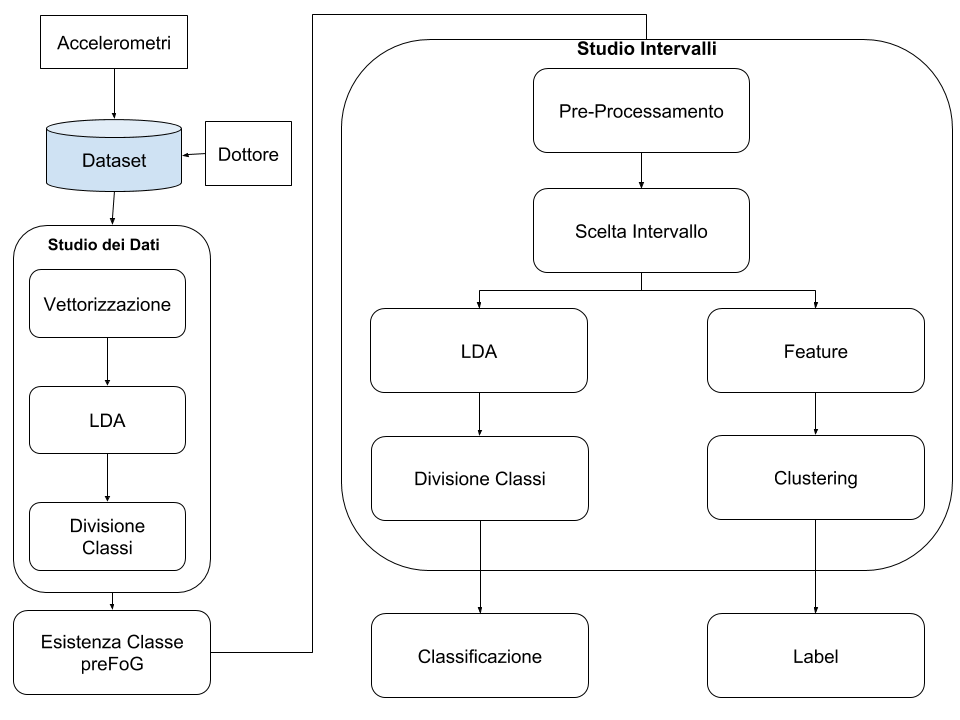
\includegraphics[scale=0.35]{images/FlussoTesi.png}
	\caption{Rappresentazione del flusso della tesi}
	\label{FlussoTesi}
\end{figure}
Lo sviluppo della tesi é stato svolto usando software Matlab.

\section{Studio sull'esistenza della classe preFOG}
Nel lavoro svolto in questa tesi si vogliono usare 3 classi invece delle 2 fornite dal dataset. Il primo passo dunque é quello di dimostrare che effettivamente le 3 classi sono distinte tra loro e che quindi sviluppare un approccio basandosi su tali classi é possibile. Per fare questo, si é usato un approccio di Discriminazione Lineare. Un discriminante é una funzione che prende in ingresso un vettore x e lo assegna ad una tra le K classi fornite. Il metodo di discriminazione che si vuole usare é quello di Fisher, il quale viene spiegato nella sezione \ref{Fisher}.\\
\subsection{Divisione dei dati}
Per ogni paziente, prendiamo in input la matrice di dati grezzi degli accelerometri fornita dal dataset, la quale contiene anche un campo relativo al tempo di ogni campione ed un'etichetta, che mi indica lo stato in cui si trova il mio paziente. Dividiamo i dati degli accelerometri da quelli relativi al tempo ed allo stato e calcoliamo delle feature su tali dati. Queste vengono calcolate vettorizzando in  finestre temporali i dati grezzi, ossia prendendo tutte le righe e colonne di un certo intervallo e disponendole lungo un vettore riga. Per tenere traccia dell'etichetta reale a cui ogni finestra temporale appartiene, abbiamo usato il vettore relativo all'etichetta fornita dal dataset e, per ogni finestra temporale, abbiamo tenuto quella che si presenta più volte all'interno di essa. Il codice implementativo di quanto appena descritto é fornito in \ref{vettorizzazione}.
\begin{lstlisting}[style=Matlab-editor,frame=single, caption=Vettorizzazione dei dati degli accelerometri, label=vettorizzazione]
for i=1:size_windows_sample-size_overlap_samples:m - size_windows_sample
B = A(i:i+size_windows_sample-1,:);
% vettorizzo ogni finestra
B=B(:);
F(number_sample,:)=B';


%salvo la classe di ogni finestra
class(number_sample)=mode(FREEZE(i:i+size_windows_sample-1,:));

%go to next sample
number_sample = number_sample + 1;

end
\end{lstlisting}
\subsection{Algoritmo di discriminazione}
Una volta vettorizzato l'intero dataset, si procede ad applicare l'algoritmo di discriminazione, il quale per prima cosa divide le feature appena calcolate tramite le classi di appartenenza. Calcola quindi la media per ogni classe e determina la dimensione di ognuna di esse. A questo punto, ricava la within class covariance e la between class covariance, ossia quanta similarità esiste tra gli elementi della stessa classe e quanta dissimilarità è presente tra classi differenti. Una volta trovate tali misure, prende gli autovalori ed autovettori della soluzione del problema dell'autovalore generalizzato e tiene solo quelli più rappresentativi, che nel caso dell'approccio di Fisher sono pari al numero di classi presenti meno 1. Questi autovalori vengono poi moltiplicati per le feature calcolate precedentemente per ottenere una riduzione della dimensionalità' ed avere 2 feature rappresentative. Il codice della discriminazione viene fornito in \ref{code_LDA}.
\begin{lstlisting}[style=Matlab-editor,frame=single, caption=LDA, label=code_LDA]
A=F';

%quindi ho A 1152x1449 double
%1152 finestre
%ogni finestra ha 1449 features
[d,N] = size(A);

K =  max(class); % numero classi in gioco;

% 1. Divido le feature tramite le classi Ck
for k = 1:K
a = find (class == k);
Ck{k} = A(:, a);
end

% 2. Calcolo la media per ogni classe per ogni finestra
for k = 1:K
mk{k} = mean(Ck{k},2);
end
% 3. Determino la grandezza di ogni classe
for k = 1:K
[d, Nk(k)] = size(Ck{k});
end
% 4. determino le within class covariance
for k = 1:K
S{k} = 0;
for i = 1:Nk(k)
S{k} = S{k} + (Ck{k}(:,i)-mk{k})*(Ck{k}(:,i)-mk{k})';
end
S{k} = S{k}./Nk(k);
end
Swx = 0;
for k = 1:K
Swx = Swx + S{k};
end

% 5. determino la between class covariance
% 5.1 determino la media totale
m = mean(A,2);
Sbx = 0;
for k=1:K
Sbx = Sbx + Nk(k)*((mk{k} - m)*(mk{k} - m)');
end
Sbx = Sbx/K;

MA = inv(Swx)*Sbx;

% eigenvalues/eigenvectors
[V,D] = eig(MA);

% 5: transform matrix
if (k > 1)
W = V(:,1:K-1);
end
if (k == 1)
W = V(:,1:1);
end

% 6: transformation
Y = W'*A;
\end{lstlisting}


\section{Etichettatura dei dati non supervisionata}
Allo stato dell'arte, sono stati condotti studi di classificazione, usando quindi dataset già etichettati da dottori. In questa sezione usiamo un approccio non supervisionato tramite clustering al fine di sostituire il medico nella fase di etichettatura dei dati, usando uno studio sulla divisione dei dati in finestre temporali, trovando così anche quale sia il miglior modo di suddividere in intervalli i nostri dati. L'approccio che è stato preso in considerazione è basato sul calcolo di feature (o proprietà) derivanti dalla matematica statistica. Il flusso di tale approccio è:
\begin{enumerate}
	\item Pre-processamento dei dati degli accelerometri, al fine di eliminare il rumore presente ed identificare eventuali punti di outline, ossia campioni che non presentano affinità col resto dei dati poiché dovuti a movimenti non consoni;
	\item Finestramento dei dati in base ad intervalli variabili al fine di calcolare le feature, dove ogni intervallo presenta una certa sovrapposizione con l'intervallo precedente;
	\item Calcolo effettivo delle feature statistiche;
	\item Applicazione degli algoritmi di clustering;
	\item Calcolo di metriche che indicano quanto bene gli algoritmi di clustering hanno diviso i dati in relazione alle label fornite dal dataset.
\end{enumerate}
\begin{figure}[h!]
	\centering
	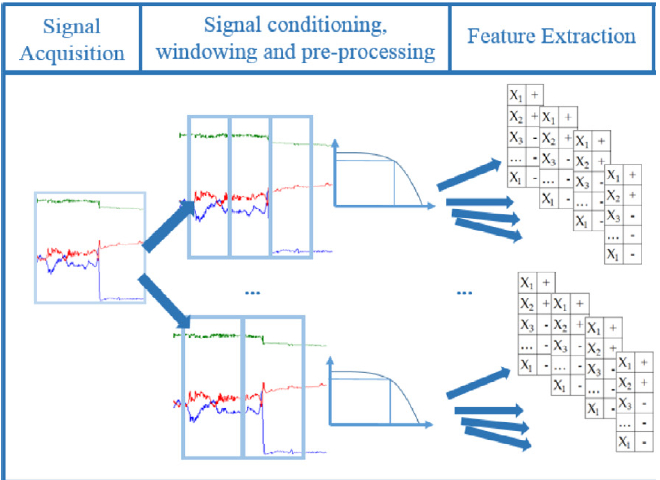
\includegraphics[scale=0.6]{images/flusso_feature.png}
	\caption{Schema generale di calcolo delle feature statistiche}
	\label{Flusso Feature}
\end{figure}
\subsection{Pre-processamento dei dati}
Gli accelerometri sono dispositivi che misurano le vibrazioni o l'accelerazione del movimento di una struttura. La forza generata dalle vibrazioni o una variazione del movimento (accelerazione) fa in modo che la massa "comprima" il materiale piezoelettrico, che genera una carica elettrica proporzionale alla forza esercitata su di esso. Dato che la carica è proporzionale alla forza e che la massa è una costante, la carica è proporzionale anche all'accelerazione. Come tutti i dispositivi che misurano delle grandezze presentano dell'incertezza strumentale che può portare ad avere rumore, ossia un segnale non desiderato, di origine naturale o artificiale, che si sovrappone all'informazione degli accelerometri stessi. Questo rumore porta ad avere dei punti definiti outlier, ossia campioni che non presentano affinità col resto dei dati poiché dovuti a movimenti non consoni.\\
Al fine di non alterare in modo negativo il calcolo delle nostre feature, si rende necessario rimuoverli dal nostro dataset. Per identificarli, è stato implementato un filtro passa-alto che elimina tutte le frequenze inferiori a 0.5Hz, le quali non appartengono al normale movimento umano ma indicano appunto la presenza di rumore, come evidenziato in \cite{21}.
\subsection{Definizione degli intervalli}
Una volta filtrati i dati, il passo successivo dell'algoritmo consiste nel dividerli in intervalli temporali, al fine di poter computare le caratteristiche degli stessi. Un intervallo contiene un determinato movimento, che però verrebbe "interrotto" con la fine della finestra stessa e quindi potrei perdere informazioni su tale movimento. Per evitare il più possibile tale perdita, viene usato un approccio che sfrutta le sovrapposizioni tra intervalli, per cui ogni nuova finestra non inizia subito dopo la fine della precedente, ma all'interno di essa. La durata degli intervalli che sono stati presi in considerazione sono:
\begin{itemize}
	\item  Da 1 secondi a 5 secondi per la finestra temporale, con un incremento di 0.5 secondi;
	\item Da 0.5 a 4.5 secondi per l'intervallo di overlap, con un incremento sempre di 0.5 secondi.
\end{itemize}
La condizione fondamentale per usare le sovrapposizioni è che l'intervallo delle stesse non sia mai maggiore della durata delle finestre temporali, per cui è stata posta la condizione che la finestra temporale sia sempre almeno 0.5 secondi più lunga dell'intervallo di sovrapposizione. Per capire da dove parte la nuova finestra, quindi, prendiamo la posizione a cui siamo arrivati e togliamo la durata della sovrapposizione. L'implementazione viene fornita in \ref{intervals}.
\begin{lstlisting}[style=Matlab-editor,frame=single, caption=Definizione degli intervalli, label=intervals]  % Start your code-block
...
for k = 5:5:45

Y = k/10;

for i = (Y+0.5):0.5:5
%dimensione della finestra in secondi
size_windows_sec = i;
%dimensione della finestra in campioni
size_windows_sample = Fs * i;

%dimensione dell'overlap in secondi
size_overlap_sec = Y;
%dimensione dell'overlap in campioni
size_overlap_samples = Fs * Y;

number_sample = 1;

%for each sample window, compute the features
for i=1:size_windows_sample-size_overlap_samples:m - size_windows_sample
B = A(i:i+size_windows_sample-1,:);
...
\end{lstlisting}
\subsection{Calcolo delle Feature}
 Per ogni possibile combinazione di finestra temporale e sovrapposizione, a questo punto vengono calcolate le feature per ogni intervallo. Le feature prese in considerazione nel nostro studio sono descritte in tabella \ref{TAB:Feature}.
\begin{table}[h!]
	\begin{tabular}{ |p{0.05\textwidth} | p{0.25\textwidth} | p{0.6\textwidth} | }
		\multicolumn{1}{|p{0.05\textwidth} |}{\textbf{N}} &  
		\multicolumn{1}{p{0.25\textwidth} |}{\textbf{Feature}} &
		\multicolumn{1}{p{0.6\textwidth} |}{\textbf{Descrizione}}\\
		\hline
		\hline
		1 & Minimo & Valore minimo del segnale\\
		2 & Massimo & Valore massimo del segnale \\
		3 & Mediana & Valore mediano del segnale \\
		4 & Media & Valore medio del segnale \\
		5 & Media Armonica & Media armonica del segnale \\
		6 & Errore Quadratico Medio & Valore Quadratico medio del segnale \\
		7 & Media Geometrica & Media geometrica del segnale \\
		8 & Varianza & Radice della deviazione standard \\
		9 & Deviazione Standard & Deviazione media del segnale rispetto alla media \\
		10 & Curtosi & Allontanamento dalla normalità distributiva del segnale \\
		11 & Simmetria & Grado di asimmetria della distribuzione del segnale \\
		12 & Moda & Il numero che appare più volte nel segnale \\
		13 & Media Tagliata & Media tagliatadel segnale nella finestra \\
		14 & Entropia & Misura della di distruzione delle componenti in frequenza \\
		15 & Range & Differenza tra il valore minimo e massimo del segnale \\
		16 & Magnitudine & Somma della norma euclidea di tre assi normalizzato sulla lunghezza del segnale \\
		17 & Area Magnitudine & Accelerazione della magnitudine di tre assi normalizzato sulla lunghezza del segnale \\
		18 & Autovalori delle direzioni dominanti & Autovalori della matrice di covarianza di tre assi \\
		19 & Accelerazione media dell'energia & Valore medio dell'energia sui 3 assi \\
	\end{tabular}
\caption{Descrizione delle Feature Statistiche}
\label{TAB:Feature}
\end{table}\\
Nel dataset, ogni campione è etichettato. Poiché le nostre feature sono composte da molti campioni messi assieme, si rende necessario trovare un metodo per unire, sbagliando il meno possibile, tutte le etichette della finestra che prendiamo in considerazione. Per fare ciò, si è deciso di utilizzare la funzione di moda, ossia il numero che si ripete più spesso all'interno dell'intervallo considerato. L'etichetta risultante viene inserita nella tabella e verrà utilizzata come criterio di confronto, al fine di valutare le prestazioni degli algoritmi di clustering. L'implementazione del codice è fornito in \ref{extract_feature}
\begin{lstlisting}[style=Matlab-editor,frame=single, caption=Calcolo delle Feature, label=extract_feature]  % Start your code-block
...
%time sample
F(number_sample, 1) = TIME(i,:);
%min --> minimum value for each accelerometer
F(number_sample, 2:10) = min(B);
%max --> maximum value for each accelerometer
F(number_sample, 11:19) = max(B);
%median --> median signal value
F(number_sample, 20:28) = median(B);
%mean --> average value
F(number_sample, 29:37) = mean(B);
%ArmMean --> harmonic average of the signal
F(number_sample, 38:46) = harmmean(B);
%root mean square --> quadratic mean value of the signal
F(number_sample, 47:55) = rms(B);
%variance --> square of the standard deviation
F(number_sample, 56:64) = var(B);
%standard deviation --> mean deviation of the signal compared to the
%average
F(number_sample, 65:73) = std(B);
%kurtosis --> degree of peakedness of the sensor signal distribution
%(allontanamento dalla normalita distributiva)
F(number_sample, 74:82) = kurtosis(B);
%skewdness --> degree of asymmetry of the sensor signal distribution
F(number_sample, 83:91) = skewness(B);
%mode --> number that appears most often in the signal
F(number_sample, 92:100) = mode(B);
%trim mean --> trimmed mean of the signal in the window
F(number_sample, 101:109) = trimmean(B,10);
%range --> difference between the largest and the smallest values of
%the signal
F(number_sample, 110:118) = range(B);
%signal magnitude vector --> sum of the euclidean norm over the three
%axis over the entire window normalized by the windows lenght
F(number_sample, 119) = svmn(B(:,1:3), length(B));
F(number_sample, 120) = svmn(B(:,4:6), length(B));
F(number_sample, 121) = svmn(B(:,7:9), length(B));
%normalized signal magnitude area --> acceleration magnitude summed
%over three axes normalized by the windows length
F(number_sample, 122) = sman(B(:,1:3), length(B));
F(number_sample, 123) = sman(B(:,4:6), length(B));
F(number_sample, 124) = sman(B(:,7:9), length(B));
%eigenvalues of dominant directions --> eigenvalues of the
%covariance matrix of the acceleration data along x, y and z axis
F(number_sample,125) = eigs(cov(B(:,1:3)),1);
F(number_sample,126) = eigs(cov(B(:,4:6)),1);
F(number_sample,127) = eigs(cov(B(:,7:9)),1);
%averaged acceleration energy --> mean value of the energy over
%three acceleration axes
F(number_sample,128) = energyn(B(:,1:3),length(B));
F(number_sample,129) = energyn(B(:,4:6),length(B));
F(number_sample,130) = energyn(B(:,7:9),length(B));
%is freezing?
F(number_sample,131) = mode(FREEZE(i:i+size_windows_sample-1,:));

%go to next sample
number_sample = number_sample + 1;
...
\end{lstlisting}
\subsection{Clustering}
Una volta finestrato il segnale, si procede con l'applicazione degli algoritmi di clustering. Quelli che sono stati presi in considerazione nella nostra analisi sono: K-means, Fuzzy C-Means e Neural Network. Il K-means viene testato in 4 varianti diverse, in base alle seguenti metriche di distanza: cityblock, correlation, cosine, euclidean.\\
Ogni algoritmo di clustering viene applicato in tutte le possibili combinazioni di intervalli ed ognuno di essi restituisce un vettore di numeri, che corrispondono alle etichette che assegnano ad ogni vettore di feature. Questi vengono salvati e verranno poi utilizzati per calcolare le prestazioni degli algoritmi stessi in confronto alla classificazione originale del medico. L'implementazione del codice è fornita in \ref{clustering}
\begin{lstlisting}[style=Matlab-editor,frame=single, caption=Uso degli algoritmi di clustering, label=clustering]  % Start your code-block
...
            %% k-means %%%

% choose of parameter
means1 = 'sqeuclidean';
means2 = 'correlation';
means3 = 'cityblock';
means4 = 'cosine';
for q=1:4
if q == 1
dist_k = means1;
end
if q == 2
dist_k = means2;
end
if q == 3
dist_k = means3;
end
if q == 4
dist_k = means4;
end
options_km = statset('UseParallel', false);
maxiter = 100000;
% cluster
kidx = kmeans(bonds, numClust, 'distance', dist_k, 'options', options_km, 'MaxIter', maxiter);

P = array2table([A(:,n) kidx]);
writetable(P, [datadir 'versus_kmeans_' dist_k '_' fileruns(r).name] );
display([datadir 'versus_kmeans_' dist_k '_' fileruns(r).name]);
end

%%% neural networks - Self organizing Maps %%%

% Create a Self-Organizing Map
dimension1 = 3;
dimension2 = 1;
net = selforgmap([dimension1 dimension2]);

% Train the network
net.trainParam.showWindow = 0;
[net,tr] = train(net,bonds');

% Test the network
nidx = net(bonds');
nidx = vec2ind(nidx)';

P = array2table([A(:,n) nidx]);
writetable(P, [datadir 'versus_net_' fileruns(r).name] );
display([datadir 'versus_net_' fileruns(r).name]);


%     %%% FUZZY C-MEANS %%%
options(1) = 2;
options(2) = 10000;
options(3) = 1e-5;
options(4) = 0;
% Hide iteration information by passing appropriate options to FCM
[centres,U] = fcm(bonds,numClust,options);
[~, fidx] = max(U);
fidx = fidx';


P = array2table([A(:,n) fidx]);
writetable(P, [datadir 'versus_cmeans_' fileruns(r).name] );
display([datadir 'versus_cmeans_' fileruns(r).name]);
...
\end{lstlisting}
\subsection{Calcolo delle prestazioni}
Ogni algoritmo di clustering, per tutte le combinazioni di finestra ed overlap, fornisce un vettore di etichette. Questo rappresenta la divisione in cluster effettuata dall'algoritmo, i quali andranno confrontati con le etichette reali del dataset. Per fare questo, procediamo al calcolo di metriche quali, in ordine, accuratezza, precisione, sensitività e F1-measure. Per quanto riguarda la precisione, la sensitività e l'F1-measure, esse sarebbero relative ad ogni classe, ma poiché ci interessa indovinare la maggior parte delle volte tutte e 3 le classi, quelle che saranno riportate sono la media dei valori per ogni classe. Il codice implementativo é fornito in \ref{rate}

\begin{lstlisting}[style=Matlab-editor,frame=single, caption=Calcolo delle prestazioni, label=rate]  % Start your code-block
...
% Matrice di confusione
[C,order] = confusionmat(D(:,2),D(:,1));
accuracy = c_accuracy(C);
precision = c_precision(C);
recall = c_recall(C);
F1measure = c_F1measure(precision,recall);

B = [accuracy precision recall F1measure];
E = [E B];

end
Q = [Q ; [e E]];
e = [e [0 0 0 0]];
...
\end{lstlisting}
Viene creata dunque una tabella che riassume, per ogni possibile intervallo, le prestazioni dell'algoritmo, come si vede in \ref{ratecluster1}, \ref{ratecluster2}, \ref{ratecluster3}.
\begin{table}[htp]
	\centering
	\caption{Esempio di tabelle delle prestazioni del clustering}
	\label{ratecluster1}
	\resizebox{\textwidth}{!}{%
	\begin{tabular}{|l|l|l|l|l|l|l|l|l|l|l|l|l|}
		\hline
		& \multicolumn{4}{c|}{Secondi: 1} & \multicolumn{4}{c|}{Secondi: 1.5} & \multicolumn{4}{c|}{Secondi: 2} \\ \hline
		Ov 0.5 & 0,7 & 0,6 & 0,3 & 0,4 & 0,8 & 0,3 & 0,3 & 0,3 & 0,91 & 0,5 & 0,5 & 0,5 \\ \hline
		Ov 1 & 0 & 0 & 0 & 0 & 0,7 & 0,3 & 0,3 & 0,3 & 0,8 & 0,6 & 0,5 & 0,55 \\ \hline
		Ov 1.5 & 0 & 0 & 0 & 0 & 0 & 0 & 0 & 0 & 0,91 & 0,72 & 0,6 & 0,6 \\ \hline
	\end{tabular}%
}
\end{table}
\begin{table}[htp]
	\centering
	\caption{Esempio di tabelle delle prestazioni del clustering}
	\label{ratecluster2}
	\resizebox{\textwidth}{!}{%
	\begin{tabular}{|l|l|l|l|l|l|l|l|l|l|l|l|l|}
		\hline
		& \multicolumn{4}{c|}{Secondi: 2.5} & \multicolumn{4}{c|}{Secondi: 3} & \multicolumn{4}{c|}{Secondi: 3.5} \\ \hline
		Ov 0.5 & 0,7 & 0,3 & 0,3 & 0,3 & 0,4 & 0,1 & 0,2 & 0,17 & 0,46 & 0,32 & 0,4 & 0,35 \\ \hline
		Ov 1 & 0,05 & 0,3 & 0,2 & 0,3 & 0,46 & 0,3 & 0,4 & 0,38 & 0,46 & 0,32 & 0,4 & 0,35 \\ \hline
		Ov 1.5 & 0,75 & 0,2 & 0,2 & 0,2 & 0,8 & 0,3 & 0,3 & 0,3 & 0,46 & 0,32 & 0,4 & 0,35 \\ \hline
		Ov 2 & 0,8 & 0,3 & 0,3 & 0,3 & 0,6 & 0,3 & 0,1 & 0,21 & 0,46 & 0,32 & 0,4 & 0,35 \\ \hline
		Ov2.5 & 0 & 0 & 0 & 0 & 0,81 & 0,26 & 0,24 & 0,25 & 0,7 & 0,3 & 0,2 & 0,26 \\ \hline
		Ov 3 & 0 & 0 & 0 & 0 & 0 & 0 & 0 & 0 & 0,6 & 0,3 & 0,31 & 0,31 \\ \hline
	\end{tabular}%
}
\end{table}
\begin{table}[htp]
	\centering
	\caption{Esempio di tabelle delle prestazioni del clustering}
	\label{ratecluster3}
	\resizebox{\textwidth}{!}{%
	\begin{tabular}{|l|l|l|l|l|l|l|l|l|l|l|l|l|}
		\hline
		& \multicolumn{4}{c|}{Secondi: 4} & \multicolumn{4}{c|}{Secondi: 4.5} & \multicolumn{4}{c|}{Secondi: 5} \\ \hline
		Ov 0.5 & 0,8 & 0,36 & 0,35 & 0,35 & 0,81 & 0,32 & 0,34 & 0,33 & 0,75 & 0,24 & 0,26 & 0,25 \\ \hline
		Ov 1 & 0,76 & 0,21 & 0,28 & 0,26 & 0,79 & 0,32 & 0,34 & 0,31 & 0,79 & 0,3 & 0,3 & 0,3 \\ \hline
		Ov 1.5 & 0,46 & 0,36 & 0,33 & 0,35 & 0,8 & 0,36 & 0,35 & 0,35 & 0,59 & 0,24 & 0,33 & 0,29 \\ \hline
		Ov 2 & 0,41 & 0,33 & 0,44 & 0,39 & 0,76 & 0,21 & 0,28 & 0,26 & 0,26 & 0,79 & 0,32 & 0,34 \\ \hline
		Ov2.5 & 0,59 & 0,24 & 0,33 & 0,29 & 0,46 & 0,36 & 0,33 & 0,35 & 0,35 & 0,8 & 0,36 & 0,35 \\ \hline
		Ov 3 & 0,44 & 0,11 & 0,12 & 0,11 & 0,41 & 0,33 & 0,44 & 0,39 & 0,8 & 0,36 & 0,35 & 0,35 \\ \hline
		Ov 3.5 & 0,78 & 0,23 & 0,33 & 0,28 & 0,75 & 0,24 & 0,26 & 0,25 & 0,76 & 0,21 & 0,28 & 0,26 \\ \hline
		Ov 4 & 0 & 0 & 0 & 0 & 0,79 & 0,3 & 0,3 & 0,3 & 0,75 & 0,24 & 0,26 & 0,25 \\ \hline
		Ov 4.5 & 0 & 0 & 0 & 0 & 0 & 0 & 0 & 0 & 0,79 & 0,3 & 0,3 & 0,3 \\ \hline
	\end{tabular}%
	}
\end{table}


\section{Classificazione del preFOG}
Nella sezione precedente, è stato decritto uno studio degli intervalli temporali che ci ha portati a decidere quale sia la migliore scelta di durata sia per la finestra che per la sovrapposizione al fine di dividere al meglio i dati a nostra disposizione. Dalla figura \ref{LDAALL2.png}, si nota come le classi FoG e NoFoG sono a volte confuse tra di loro, mentre il preFOG è più o meno diviso dalle altre due classi. Ma quest'ultima classe è proprio quella che stiamo studiando ed è quella che ci porterebbe a prevenire le occorrenze di FoG, in quanto, identificandola, avrei il tempo di dare lo stimolo prima dell'avvenuta del FoG, mentre se cerco di identificare solo i Freezing darei lo stimolo uditorio in ritardo in ogni caso. Questo ci porta a provare un primo approccio di classificazione a 2 classi, dove raggruppiamo assieme i dati di FoG e noFoG e teniamo separate le occorrenze di preFOG. L'algoritmo  di classificazione scelto è il K-nearest Neighbours (KNN), spiegato nel capitolo \ref{chap3:background}. Usiamo sempre l'intervallo che è stato dimostrato nella sezione precedente essere quello più affidabile. L'algoritmo verrà testato in due modi:
\begin{itemize}
	\item alleniamo il knn su un paziente singolo, effettuiamo una cross-validation sul classificatore e lo testiamo su dei nuovi dati, ossia che non sono stati inclusi nella  cross-validation;
	\item alleniamo il knn sui dati di tutti i pazienti contemporaneamente ed effettuiamo una cross-validation.
\end{itemize}
La cross-validation è una tecnica statistica utilizzabile in presenza di una buona numerosità del campione osservato o training set. In particolare la k-fold cross-validation consiste nella suddivisione del dataset totale in k parti di uguale numerosità (si chiama anche k-fold validation) e, ad ogni passo, la k-esima parte del dataset viene ad essere il validation dataset, mentre la restante parte costituisce il training dataset. In altre parole, si suddivide il campione osservato in gruppi di egual numerosità, si esclude iterativamente un gruppo alla volta e lo si cerca di predire con i gruppi non esclusi.\\
Il codice implementativo viene fornito in \ref{validation}

\begin{lstlisting}[style=Matlab-editor,frame=single, caption=Cross-Validation, label=validation]  % Start your code-block

% Cross-Validation
cp = cvpartition(y,'k',10);

f = @(xtr,ytr,xte,yte)confusionmat(yte,...
classify(xte,xtr,ytr),'order',order);

cfMat = crossval(f,X,y,'partition',cp);
cfMat = reshape(sum(cfMat),2,2)
...
% Previsione nuovi dati
[label,~,~] = predict(Mdl_LDA,Y1');
[C,~] = confusionmat(classi,label)

CP = classperf(classi,label);
rate = [CP.CorrectRate CP.Sensitivity CP.Specificity CP.F1measure]
\end{lstlisting}